\section{International Strategy}
%Using the examples of Google, Apple, Samsung, Boeing and Airbus strategies of the large~\mne~have extended. 
%It is no longer just resources and industries that dictate the strategies that companies employ. 
%According to~\cite{Peng:2009vt}, the market-based institutional framework has been taken for granted, and formal institutions (such as laws and regulations) and informal institutions (such as cultures and norms) have been assumed away as``background''.\\
%This trend has given rise to what~\cite{Peng:2009vt} calls the `third leg' of the strategy tripod.
%~\Gls{IBV} has been an addition to the theories of~\gls{RBV} introduced by~\cite{Barney:1991ur} and industry based view by~\cite{Porter:1980to}. 

Since being introduced by~\citep{Porter:1980to} the `industry based view' and \gls{RBV}~\citep{Barney:1991ur}~have gained a lot of momentum in the international business community.
Strategic management (theory) or strategy in short has become a household name.
In the following sections the theories of~\citep{Barney:1991ur,Barney:2011jp} will be discussed briefly, followed by a more extensive discussion on~\ibv.
As the \rbt~is the prevailing theory in this thesis, this theory will be discussed more extensively.
As \rbt~is not the only important IB theory and \rbt~is closely linked to \inbv~and to a lesser extend \ibv.
Both other theories are discussed in Appendix~\ref{Ch:Porter} and~\ref{ch:peng} respectively.

\subsection{Resourced Based Theory}\label{sec:Barney} % Section voor Barney

\Gls{RBV} came as a response to \gls{InBV} by~\cite{Porter:1980to}.
\Gls{RBV} has been introduced by among others~\cite{Barney:1991ur,Wernerfelt:1984hx}
Nowadays more and more scholars are using the term \rbt.
\begin{quote}
  scholars are increasingly using the term resource-based theory instead of
resource-based view.
This reflects the fact that resource-based research has reached a level of
precision and sophistication such that it more closely resembles a theory than a 
view~\citep{Barney:2011jp}.
\end{quote}
The term \rbt for the theory of~\cite{Barney:1991ur,Barney:2011jp} will also be used in this thesis.

Contrary to~\cite{Porter:1980to}, \rbt researched the link between firm's internal characteristics and it's performance~\citep{Barney:1991ur}.\\
A key concept is that \rbt assumes that (a) firms across one industry may be heterogeneous with respect to strategic resources and (b) that resources are not perfectly mobile across firms, hence heterogeneity may be long lasting~\citep{Barney:1991ur}.
%The key assumptions in \rbt (and thus \rbv) are that (a) firms within an industry may be heterogeneous with respect to the strategic resources they control and (b) these resources are may not be perfectly mobile across firms.
%This makes that the heterogeneity can be long lasting~\cite{Barney:1991ur}.
%\Gls{RBV} argues that a firms strategic advantage is depended on it's heterogeneous resources (a bundle of all assets, knowledge, and capabilities) which have to be the following:

The \glsfull{RBT} argues that firms posses resources, a subset of which enables them to achieve competitive advantage and a further subset which leads to superior long-term performance~\citep{Barney:1991ur,Wernerfelt:1984hx,Grant:1991wg}.
Studies of firm performance using \glsfull{RBT} have found differences not only between firms in similar industry but also within narrower groups within 
industries~\citep{Hansen:1989um,Cool:1988vw}.
The resources that are mentioned are defined as \textit{assets and capabilities that are available and useful in detecting and responding to market opportunities or threats}~\citep{sanchez:1996,Wade:2004wf}.
Where \textit{assets} are `anything tangible or intangible the firm can use in it's processes for creating, producing and/or offering it's products (or services) to a market'~\citep{sanchez:1996}.
\textit{Capabilities} have been defined as `repeatable patterns of actions in the use of assets to create produce and/or offer products to a market'~\citep{sanchez:1996}.\\
The theory by~\cite{Barney:1991ur} has been captured by the acronym VRIN\@.
With the acronym VRIN, he is referring to the characteristics of the resources that are the difference makers in the business organisations.
This acronym can be explained using the itemisation below:

\begin{enumerate}[(I)]
   \setlength{\itemsep}{1pt}
\item must be valuable, in the sense that it exploit opportunities and/or neutralises threats in a firm’s environment
\item must be rare among a firm’s current and potential competition 
\item must be imperfectly imitable
\item  there cannot be strategically equivalent substitutes for this resource that are valuable but neither rare or imperfectly imitable 
\end{enumerate} 

 
Later~\cite{Oliver:1997wj} added to the \rbt~by providing the following definition:
\begin{quote}
A resource-based view proposes that resource selection and accumulation are a function of both within-firm decision-making and external strategic factors~\citep{Oliver:1997wj}.
\end{quote}
This unique combination of resources will lead to~\ca~\citep{Barney:1991ur}. \\
\rbt is not without critiques~\citep{Narayanan:2005wy,Kraaijenbrink:2009bu,Priem:2001vd,Dung:2012wh}.
A more extensive overview of the critiques on~\citep{Barney:1991ur} can be found in Appendix~\ref{app:critiques_barney}.\\
In his paper 2011 paper~\cite{Barney:2011jp} concludes that \rbt~and therefore also \rbv~is not on the decline.
\rbt~is still in use in recently published papers.
This speaks volume about on fact that this theory can still be considered relevant~\citep{Mukherjee:2013vz,Hoskisson:2012jk,Lockett:2013jr}.

\begin{figure}[htbp] 
	\centering
	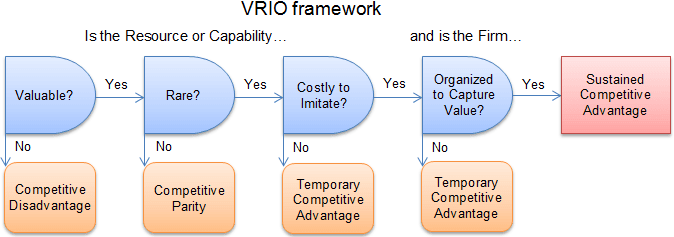
\includegraphics[width=0.8\textwidth]{vrio_framework}
 	\caption[The VRIO framework]{The VRIO framework. Adapted from~\citep{rothaermel2012strategic}}\label{fig:VRIO}
\end{figure}

The VRIN framework developed in~\cite{Barney:1991ur} was also extended and improved upon~\citep{Barney:1995tz} just as he had improved on the terminology of \rbt.
\cite{Barney:1995tz} introduced the concept of \acrshort{VRIO} to improve on \acrshort{VRIN}
\begin{description} 
   \setlength{\itemsep}{1pt}
\item[The Question of Value] Resources are valuable if they help organisations to increase the value offered to the customers. This is done by increasing differentiation or/and decreasing the costs of the production. The resources that cannot meet this condition, lead to competitive disadvantage.

\item[The Question of Rarity] Resources that can only be acquired by one or few companies are considered rare. When more than few companies have the same resource or capability, it results in competitive parity.

\item[The Question of Imitability] A company that has valuable and rare resource can achieve at least temporary competitive advantage. However, the resource must also be costly to imitate or to substitute for a rival, if a company wants to achieve sustained competitive advantage.

\item[The Question of Organisation] The resources itself do not confer any advantage for a company if it’s not organised to capture the value from them. Only the firm that is capable to exploit the valuable, rare and imitable resources can achieve sustained competitive advantage\footnote{adopted from~\citep{Strategic-management-insight:2013}}.
\end{description}

The key improvement to the VRIO (see also~\ref{fig:VRIO}) framework from the VRIN framework is the addition of the question if the organisation is ready and capable to exploit all the resources~\citep{Barney:1995tz,Strategic-management-insight:2013}.
The general thinking is this should lead to~\ca through \gls{FSA}~\citep{Barney:1991ur,Barney:2001tj,Barney:2011jp}. 
The frameworks by~\cite{Barney:1991ur,Barney:1995tz} lead to the following \wpro:

\begin{WP}\label{wp:rbt}
  The diversity in internal resources (humans and knowledge) within firms could be responsible for the heterogeneity of firms responses to changes institutional environment
\end{WP}

\subsection{Firm specific resources}

A key concept of~\citep{Barney:1991ur,Barney:2001tj} is that the different (internal) resources lead to~\glspl{FSA}.
The resources of MNE are by definition located in the host and home country of that MNE\@. 
\cite{Barney:1991ur,Barney:1995tz} suggests that ``resources within the firm are not perfectly mobile across firms and that heterogeneity can be long lasting''~\citep{Barney:1991ur}.
Whether this assumption holds true is a matter of discussion.
The fact that resources might be (perfectly) mobile given certain constraints has been brought up~\citep{Lavie:2006up,Priem:2001vd} already.\\
\cite{Hu:1995vg} identified that the firm's advantages are indeed transferable, be it with varying amounts of success (certain constraints).
The success can be made visible through the expansion of Hong Kong based firms in East Asia~\citep{Hu:1995vg}.
However the accomplishments of the same firms in their expanse into the US or Great Britain yielded a very different story~\citep{Hu:1995vg}.\\
The same holds for (high-tech) Korean firms expanding to \glsfull{EE} vis-a-vis expanding to  \glsfull{AE}. 
Different strategies were observed while sill dealing with comparable MNEs~\citep{Erramilli:1997wu}.
The same firm specific resources were employed in different capacities relative to the market that was entered.\\
Not only the economic regions that are entered are relevant to the methods and impact resources have on the MNE\@.
The type of resource has a profound effect on its capacity to be either internationally mobile or immobile~\citep{Tseng:2007wm}.\\
Some \glspl{FSA}, in the form of resources, have different characteristics in general. 
\cite{Rugman:2001ti} differentiates between three types of resources.
\begin{enumerate}[(a)]
   \setlength{\itemsep}{1pt}
\item Non location bound \fsa
\item Location bound \fsa 
\item Subsidiary specific advantages
\end{enumerate}
Where the (non) location bound \fsa are in it self to be exploited globally and easy to diffuse locally (a) or hard to exploit globally and provide local national responsiveness (b) the subsidiary specific advantages are a different matter by itself. 
They are easy to deploy globally but difficult to exploit internally~\citep{Rugman:2001ti}.
The subsidiary specific advantages display characteristics of perfectly mobile resources as they are very mobile across firms, but not within firms or MNEs.\\
The observations above relax the statement of~\cite{Barney:1991ur} somewhat as to the perfect mobility of resources.
According to~\citep{Rugman:2001ti,Tseng:2007wm,Erramilli:1997wu,Hu:1995vg,Rugman:1992uj} some consideration has to be given to the fact that resources are perfectly immobile according to \rbt.
This may not be always a certainty and depends off course, on a case by case basis as indicated above.
 
%The theory of Barney is \emph{introspective}. 
%It takes into account what is happening inside the firm.
%What knowledge is available, the people matter. 
%Processes that have been created over time are a contributing factor. 
%In the 1970's Toyota engineered \gls{tpm} for it's factories this gave them \gls{CA} over their US rivals as production cost were lower for their products.
%Only if these resources cannot be imitated in an other country and location this can create a \gls{CA}.
%In contrast to~\gls{RBV} the theory of~\cite{Porter:1980to} is thus~\emph{extrospective} and does not consider the company itself.\\
%Actually both theories are not mutually exclusive. They are very well capable of existing simultaneously. 
%This line of thought give rise to the fact that there might be a third pillar in strategy thinking.